% Frontiers template Version 2.4 Generated 2014/03/12 %%%
\documentclass{frontiersSCNS} % for Science articles

%\setcitestyle{square}
\usepackage{url,lineno}
\usepackage[english]{babel}

\DeclareFontShape{OT1}{cmtt}{bx}{n}{<5><6><7><8><9><10><10.95><12><14.4><17.28><20.74><24.88>cmttb10}{}



\newcommand{\tp}{$3^\prime${ }}
\newcommand{\fp}{$5^\prime${ }}

\linenumbers

\copyrightyear{}
\pubyear{}

\def\journal{Genetics}%%% write here for which journal %%%
\def\DOI{} \def\articleType{Methods}
\def\keyFont{\fontsize{8}{11}\helveticabold }
\def\firstAuthorLast{Lawrence
  {et~al.}} %use et al only if is more than 1 author
\def\Authors{Travis J. Lawrence\,$^{1}$, Kyle T. Kauffman\,$^{2}$,
  Katherine C.H. Amrine\,$^{1,3}$, Dana L. Carper\,$^{1}$, Raymond
  S. Lee\,$^{4}$, Peter J.  Becich\,$^{2}$, Claudia J. Canales\,$^{4}$
  and David H. Ardell\,$^{1,2*}$} \def\Address{
  $^{1}$Quantitative and Systems Biology Program, University of California, Merced, CA, USA \\
  $^{2}$Molecular Cell Biology Unit, School of Natural Sciences, University of California, Merced, CA, USA \\
  $^{3}$Dept. of Viticulture and Enology, University of California, Davis, CA, USA \\
  $^{4}$School of Engineering, University of California, Merced, CA,
  USA} \def\corrAuthor{David H. Ardell} \def\corrAddress{Molecular
  Cell Biology Unit, School of Natural Sciences, University of
  California, Merced, 5200 North Lake Road, Merced, CA , 95343, USA}
\def\corrEmail{dardell@ucmerced.edu}

\begin{document}
\onecolumn
\firstpage{1}

\title[FAST: FAST Analysis of Sequences Toolbox]{FAST: FAST Analysis of Sequences Toolbox}
\author[\firstAuthorLast ]{\Authors}
\address{}
\correspondance{}
\topic{}

\maketitle

\begin{abstract}
  FAST (FAST Analysis of Sequences Toolbox) provides simple, powerful
  open source command-line tools to filter, transform, annotate and
  analyze biological sequence data. Modeled after the GNU (GNU's Not
  Unix) Textutils such as {\tt grep}, {\tt cut}, and {\tt tr}, FAST
  tools such as {\tt fasgrep}, {\tt fascut}, and {\tt fastr} make it
  easy to rapidly prototype expressive bioinformatic workflows in a
  compact and generic command vocabulary.  Compact combinatorial
  encoding of data workflows with FAST commands can simplify the
  documentation and reproducibility of bioinformatic protocols,
  supporting better transparency in biological data science. Interface
  self-consistency and conformity with conventions of GNU, Matlab,
  Perl, BioPerl, R and GenBank help make FAST easy and rewarding to
  learn.  FAST automates numerical, taxonomic, and text-based sorting,
  selection and transformation of sequence records and alignment sites
  based on content, index ranges, descriptive tags, annotated
  features, and in-line calculated analytics, including composition
  and codon usage.  Automated content- and feature-based extraction of
  sites and support for molecular population genetic statistics makes
  FAST useful for molecular evolutionary analysis. FAST is portable,
  easy to install and secure thanks to the relative maturity of its
  Perl and BioPerl foundations, with stable releases posted to
  CPAN. Development as well as a publicly accessible Cookbook and Wiki
  are available on the FAST GitHub repository at
  \url{https://github.com/tlawrence3/FAST}.  The default data exchange
  format in FAST is Multi-FastA (specifically, a restriction of
  BioPerl FastA format).  Sanger and Illumina 1.8+ FastQ formatted
  files are also supported. FAST makes it easier for non-programmer
  biologists to interactively investigate and control biological data
  at the speed of thought.\tiny \keyFont{
  \section{Keywords:} Unix philosophy, MultiFASTA, pipeline,
  bioinformatic workflow, open source, BioPerl, regular expression,
  NCBI Taxonomy}
\end{abstract}

\section{Introduction}

Bioinformatic software for non-programmers is traditionally
implemented for user convenience in monolithic applications with
Graphical User Interfaces
(GUIs)~\citep{Smith1994,stothard_sequence_2000,Rampp2006,
  Librado01062009,waterhouse_jalview_2009,gouy2010seaview}.  However,
the monolithic application paradigm is easily outscaled by today's big
biological data, particularly Next Generation Sequencing (NGS) data at
gigabyte- and terabyte-scales. Better empowerment of non-programmers
for genome-scale analytics of big biological data has been achieved
through web-based genome browser
interfaces~\citep{Cunningham28012015,Rosenbloom28012015,Markowitz01012014}. On
the other hand, for smaller datasets, sequence and alignment editor
applications encourage manual manipulation of data, which is
error-prone and essentially irreproducible. To reduce error and
increase reproducibility in the publishing of bioinformatic and
biostatistical protocols it is important to facilitate the
documentation and automation of data science workflows through scripts
and literate programming facilities~\citep{knuth1984literate} such as
emacs org-mode~\citep[\url{http://orgmode.org}, as demonstrated in, for example][]{delescluse_making_2012} that both completely
document and encode scientific workflows for machine processing of
biological data.

Reproducibility in bioinformatics and biostatistics protocols is
crucial to maintaining public trust in the value of its investments in
high-throughput and high-dimensional measurements of complex
biological
systems~\citep{BaggerlyCoombes2009,hutson2010data,Baggerly01052011,Huang01072013}.
In one analysis, only two of 18 published microarray gene-expression
analyses were completely reproducible, in part because key analysis
steps were made with proprietary closed-source
software~\citep{Ioannidis:2008cr}. Furthermore, even though analytical
errors are a major source of retractions in the scientific
literature~\citep{Casadevall01092014}, peer-review and publication of
scientific data processing protocols is generally not yet required to
publish scientific studies.  Adequate documentation of bioinformatic
and biostatistical workflows and open source sharing of code upon
publication~\citep{Peng01072009} facilitates crowd-sourced
verification, correction and extension of code-based
analyses~\citep{barnes2010publish,Morin13042012}, and reuse of
software and data to enable more scientific discovery returns from
public data~\citep{Peng02122011}. Peer review and publication of the
data science protocols associated to scientific studies stems
temptation to overinterpret results and encourages more objectivity in
data science~\citep{Boulesteix01022010}. The ultimate remedy for these
problems is to expand literacy in modern computational and statistical
data science for science students in
general~\citep{Morin13042012,Joppa17052013}.

Web-based open-source workflow suites such as Galaxy~\citep{galaxy14},
Taverna~\citep{CPE:CPE993} and BioExtract~\citep{Lushbough01072011}
are a recent innovation in the direction of greater reproducibility in
bioinformatics protocols for genome-scale analytics. However, the most
powerful, transparent and customizable medium for reproducible
bioinformatics work is only available to bioinformatics specialists
and programmers through Application Programming Interfaces (APIs) such
as BioPerl and Ensembl~\citep{Yates01012015}. 

Yet workflow design suites and programming APIs require dedication and
time to learn.  There is a need for more bioinformatics software
in between GUIs and APIs, that empowers non-programmer scientists and
researchers to interactively and reproducibly control, process and
analyze their data without manual interventions. Closer inspection of
data and interactive construction and control of data workflows makes
it so much easier to rapidly prototype error-free workflows, nipping
errors in the bud that can completely confound downstream analyses.
In scientific computing, the time-tested paradigm for rapid
prototyping of reproducible data workflows is the Unix command-line.

In this tradition we here present FAST: FAST Analysis Sequences
Toolbox, modeled after the standard Unix toolkit~\citep{Peek2001}, now
called Coreutils.  The FAST tools follow the Unix philosophy to ``do
one thing and do it well'' and ``write programs to work
together.''~\citep{Stutz2000}. FAST workflows are completely
automated; no manual interventions to data are required.  FAST falls
between a GUI and an API, because it is used through a Command-Line
Interface (CLI).  Although the FAST tools are written in Perl using
BioPerl packages~\citep{Stajich2002}, FAST users do not need to be
able to program Perl or know BioPerl. FAST users only need basic
competence in Unix and the modest skill to compose command pipelines
in the Unix shell.  FAST therefore supports an emerging movement to
empower non-programmer biologists to learn Unix for scientific
computing. Books and courses in this emerging market include the
recent ``UNIX and Perl to the Rescue!''~\citep{bradnam2012unix} and
the Software Carpentry and Data Carpentry Foundations
workshops~\citep{wilson_software_2014}.

Unix command pipe-lines are the paradigmatic example of the ``pipes
and filters'' design pattern that embodies serial processing of data
through sequences of modular and reuseable computations. The ``pipes
and filters'' design pattern is a special case of component-based
software engineering~\citep{mcilroy_mass-produced_1969} and a core
paradigm in software
architecture~\citep{garlan_introduction_1994}. The component-wise
organization of FAST affords access to an infinite variety of
customizable queries and workflows on biological sequence data using a
small command vocabulary and combinatorial logic. Component-based
software is easier to learn, maintain and extend. It also makes it
easy for users to interactively develop new protocols through the
modular extension and recombination of existing protocols. As shown
from the examples below, non-trivial computations may be expressed on
a single line of the printed page. Thus, FAST can help empower
non-biologist programmers to develop and communicate powerful and
reproducible bioinformatic workflows for scientific investigations and
publishing.

Open-source command-line utilities for bioinformatics such as the
EMBOSS package~\citep{Rice2000}, the FASTX tools~\citep{fastx} or the
scripts that come with BioPerl~\citep{Stajich2002} typically offer
suites of tools with simple, well-defined functions that lend
themselves to scripting, but are not necessarily designed according to
the Unix toolbox philosophy specifically to interoperate through
serial composition over pipes. Similarly, FaBox~\citep{MEN:MEN1821} is
a free and open online server with functions that overlap with FAST
tools, but is not designed for serial composition. On the other hand,
the Unix toolbox model has been used before in more or less more
specialized bioinformatics applications such as the popular SAMTools
suite~\citep{Li15082009} and in the processing of NMR
data~\citep{delaglio1995nmrpipe}. A toolsuite called bp-utils, with a
similar design philosophy and some overlapping functionality with
FAST, has recently been released
at~\url{http://diverge.hunter.cuny.edu/labwiki/Bioutils}.

We have written extensive documentation for each FAST utility along
with useful error messages following recommended
practice~\citep{Seemann2013}. FAST is free and open source; its code
is freely available to anyone to re-use, verify and extend through its
GitHub repository.

\section{Design and Implementation of FAST Tools}
\subsection{The FAST Data Model}

The Unix Coreutils paradigm allows users to treat plain-text files and
data streams as databases in which {\it records} correspond to single
lines containing {\it fields} separated by {\it delimiters} such as
commas, tabs, or strings of white-space characters.  FAST extends this
paradigm to biological sequence data, allowing users to treat
collections of files and streams of multi-line sequence records as
databases for complex queries, transformations and analytics. The
Coreutils model is generalized exactly by FAST because it models
sequence record {\it descriptions} as an ordered collection of {\it
  description fields} (see below).

Another design feature of Unix tools that also characterizes the FAST
tools is their ability to accept input not only from one or more files
but also from what is called {\it standard input}, a data-stream
supported by the Unix shell, and to output analogously to {\it
  standard output}. It is this facility that allows FAST tools to be
serially composed in Unix {\it pipelines} that compactly represent an
infinite variety of expressive bioinformatic workflows. 

The default data exchange format for FAST tools is the universally
recognized FastA format~\citep{lipman1985rapid}. While no universal
standard exists for this format, for FAST, ``FastA format" means what
is conventionally called ``multi-fasta" format of sequence or alignment
data, largely as implementated in BioPerl in the module {\tt
  Bio::SeqIO::fasta}~\citep{Stajich2002}.

In the FAST implementation of FastA format, multiple sequence records
may appear in a single file or input stream. Sequence data may contain
gap characters. The logical elements (or fields) of a sequence record
are its {\it identifier}, its {\it description} and its {\it
  sequence}. The identifier (indicated with {\tt id} in the
illustration below) and description ({\tt desc}) together make the
{\it identifier line} of a sequence record, which must begin with the
sequence record start symbol {\tt >} on a single line. The description
begins after the first block of white-space on this line (indicated
with {\tt <space>}). The {\it sequence} of a record appears
immediately after its identifier line and may continue over multiple
lines until the next record starts.

In FAST, users may alter how description fields are defined in
sequence records by using Perl-style {\it regular expressions} to
define delimiters (indicated by {\tt <delim>}). FAST uses one-based
indexing of description fields.

The FAST data model is illustrated as follows:

\begin{verbatim}
>seq1-id<space>seq1-desc-field1<delim>seq1-desc-field2<delim>...
seq1-sequence
seq1-sequence
...
seq1-sequence
>seq2-id<space>seq2-desc-field1<delim>seq2-desc-field2<delim>...
seq2-sequence
seq2-sequence
...
seq2-sequence
\end{verbatim}

In FAST, the sequence identifier is thought as the zero$^{th}$ field
of the identifier line. One-based indexing of description fields in
FAST is therefore consistent with zero-based indexing in Perl and
one-based indexing of sequence coordinates, making all indexing
consistent and uniform in FAST.

Most FAST tools extend the field-based paradigm further by supporting
{\it tagged values} in sequence record descriptions. Tagged values are
name-value pairs with a format ``name=value" as common in General
Feature Format (GFF) used in sequence annotation (see
e.g. \url{https://www.sanger.ac.uk/resources/software/gff/}) or an
alternative ``name:value'' format that certain FAST tools themselves
can append to sequence records. Support for tagged values in FAST makes it
possible to operate on sequence records with unordered or
heterogeneous description fields.

\subsection{Overview of the FAST Tools}

FAST utilities may be assigned to categories according to their
default behavior and intended use. There are FAST tools for {\bf
  selection} of data from sequence records, {\bf transformation} of
data, {\bf annotation} of sequence record descriptions with computed
characteristics of the data, and {\bf analysis}.  A complete
description of all utilities included in the first major release of
FAST is shown in Table~\ref{tab:01}.

\begin{table}[!t]
\textbf{\refstepcounter{table}\label{tab:01} Table \arabic{table}.}{
  Utilities in first major release of FAST}

\processtable{ }
{\begin{tabular}{llll}\toprule
    Tool/Category  & Function  & Coreutil analog & Operates by default
    upon \\
 \hline
  \multicolumn{4}{l}{{\bf Selection}} \\
  \hline
    {\tt fasgrep} & regex selection of records & {\tt grep} & identifiers\\
    {\tt fasfilter} & numerical selection of records &  & identifiers \\
    {\tt fastax} & taxonomic selection of records &  & descriptions \\
    {\tt fashead} & order-based selection of records & {\tt head} & records \\
    {\tt fastail} & order-based selection of records &  {\tt tail}  & records \\
    {\tt fascut} & index-based selection and reordering of data  &    {\tt cut}  & sequences \\
    {\tt gbfcut} & extract sequences by regex matching on features  & & features\\
    {\tt alncut} & selection of sites by content &  & sites \\
    {\tt gbfalncut} & selection of sites by features &  & sites \\
 \hline
  \multicolumn{4}{l}{{\bf Transformation}} \\
  \hline    
   {\tt fassort} & numerical or text sorting of records  & {\tt sort} & sequences\\
    {\tt fastaxsort} & taxonomic sorting of records &  & descriptions
    \\
    {\tt fasuniq} & remove or count redundant records & {\tt uniq} & sequences \\
    {\tt faspaste} & merging of records &  {\tt paste} & sequences \\
    {\tt fastr} & character transformations on records & {\tt tr} & identifiers\\
    {\tt fassub} & regex substitutions on records &  & identifiers \\
    {\tt fasconvert} & convert sequence formats &  &  records \\
\hline
  \multicolumn{4}{l}{{\bf Annotation}} \\
  \hline    
    {\tt faslen} & annotate sequence lengths &  & descriptions \\
    {\tt fascomp} & annotate monomeric compositions &  & descriptions \\
    {\tt fascodon} & annotate codon usage &  & descriptions \\
    {\tt fasxl} & annotate biological translations &  & descriptions \\
    {\tt fasrc} & annotate reverse complements &  & descriptions \\
\hline
  \multicolumn{4}{l}{{\bf Analysis}} \\
  \hline   
    {\tt alnpi} & molecular population genetic statistics &  &  sites \\
    {\tt faswc} & tally sequences and characters & {\tt wc} &   sequences \\
  \hline   
\end{tabular}}{}
\end{table}

The {\bf analysis} class is distinguished from the other classes
because by default, these utilities output tables of plain-text data
rather than sequence record data in FastA format. Two other tools,
{\tt fasconvert} and {\tt gbfcut}, are designed to either input or
output FastA format sequence records by default. Standardization of
the FAST data model allows users to serially compose FAST tools into
pipelines at the Unix command-line, which is indicated as the ``main
workflow'' in the overview of the project shown in
Figure~\ref{fig:01}.

\subsection{General Implementation and Benchmarking}

The BioPerl backend of FAST 1.x is version 1.6.901 downloaded in
January, 2012. {\tt Bio::SeqIO} components were updated to version 1.6.923
on June 4, 2014 and some Bio::Root components were updated on July 10,
2014 (github commit 50f87e9a4d).  We introduced a small number of
customizations to the BioPerl code-base, primarily to
enable the translation of sequences containing gaps. All of the
BioPerl dependencies of FAST are isolated under its own FAST
name-space.

To help reduce the overall installation footprint of FAST, BioPerl
dependencies of FAST scripts were analyzed with the Cava packager
(\url{http://www.cavapackager.com}).

Nearly all FAST utilities process sequence records inline and
therefore have linear runtime complexity in the number of
sequences. Exceptions are {\tt fassort} and {\tt fastail} which both
require some paging of data into temporary files. We performed
benchmarking of FAST tools using randomly generated sequences of even
composition sourced generated in Python and the {\tt Benchmark} v1.15
Perl module on a MacBook Pro 2.5 Ghz Intel i7, with 8 Gb of RAM. We
examined average CPU runtime over 100 replicates, comparing input
sizes of 25K, 250K, or 1M sequence records of length 100, 10K, 100K,
or 1M bp. Our benchmarking results show that despite data paging, {\tt
  fassort} runtimes scale linearly with input size (fig~\ref{fig:02}).

FAST is not designed to be fastest at computing its
solutions. Rather the fastness of FAST lies in how quickly an adept
user can interactively prototype, develop, and express bioinformatic
workflows with it.

\subsection{Installation and Dependencies}
FAST requires a working Perl installation, with official releases
distributed through the Comprehensive Perl Archive Network (CPAN). A
small footprint of BioPerl dependencies has been packaged together in
the FAST namespace. Other CPAN dependencies may be detected and
installed by the {\tt cpan} package manager. A fully automated install
from CPAN may on many systems be initiated by executing {\tt perl
  -MCPAN -e 'install FAST'}. A manual install follows standard Perl
install procedure. After downloading and unpacking the source
directory, change into that directory and execute: {\tt perl
  Makefile.PL; make; make test; (sudo) make install}.

We recommend that first-time users first complete the automated
install from CPAN which will handle prerequisites, and then download
and open the source code directory in order to practice the example
usage commands (such as those in the sequel) on sample data provided
within.

\subsection{Implementation and Usage of Individual Tools}

Further implementation and usage details of individual FAST tools
follows. Usage examples for individual tools refer to example data
that ships with the FAST source-code installer, available from CPAN.
The most recent version at the time of publication is 1.06, available
from \url{http://search.cpan.org/~dhard/FAST-1.06/}. These usage
examples should be able to run from within the installation directory
after installation has completed.

%\subsubsection{{\bf {\tt fasgrep}}} 
\begin{description}
\item[\texttt{ \textbf{fasgrep}} ] supports {\it regular
    expression}-based selection of sequence records. FAST uses
  Perl-style regular expressions, which are documented freely online
  and within Perl, and are closely related to Unix extended regular
  expressions. For reference on Perl regular expressions, try
  executing {\tt man perlre} or {\tt perldoc perlre}.  For example, to
  print only protein sequences that do {\it not} start with M for
  methionine, execute:
\begin{verbatim}
     fasgrep -s -v "^M" t/data/P450.fas
\end{verbatim}
  \noindent In the above command the {\tt -s} option directs {\tt
    fasgrep} to search the sequence data of each record. The {\tt -v}
  option directs {\tt fasgrep} to print records that {\it do not}
  match the pattern given by its argument, which is the regular
  expression \verb|^M|, in which the {\it anchor} \verb|^| specifies
  the beginning of the sequence data. {\tt fasgrep} uses the BioPerl {\tt
    Bio::Tools::SeqPattern} library to support ambiguity expansion of
  IUPAC codes in its regular expression arguments. Thus, to show that
  a segment of {\it Saccharomyces cerevisiae} chromosome 1 contains at
  least one instance of an ``Autonomous Consensus Sequences''
  characteristic of yeast origins of
  replication~\citep{leonard_dna_2013}, look whether the following
  command outputs a sequence or not:
\begin{verbatim}
     fasgrep -se 'WTTTAYRTTTW' t/data/chr01.fas
\end{verbatim}
\noindent which is equivalent to: 
\begin{verbatim}
     fasgrep -se '[AT]TTTA[CT][AG]TTT[AT]' t/data/chr01.fas
\end{verbatim}
\noindent These examples demonstrate queries on sequence data, but
{\tt fasgrep} may be directed to search against other parts of
sequence records including identifiers, descriptions, fields and
more.
\\
\item[\texttt{ \textbf{fasfilter}} ] supports precise numerical-based
selections of sequence records from numerical data in identifiers,
descriptions, fields or tagged-values in descriptions. {\tt fasfilter}
supports {\it open ranges} such as {\tt 100-}, meaning ``greater than or
equal to 100'', closed ranges like {\tt 1e6-5e8} (meaning $1 \times
10^{6}$ to $5 \times 10^{8}$) and compound ranges
such as {\tt 200-400,500-}. Ranges may be specified in Perl-style (or
GenBank coordinate style) like {\tt from..to}, in R/Octave-style like
{\tt from:to} or UNIX {\tt cut}-style as in {\tt from-to}. For
example, to print records with gi numbers between 200 million and 500
million, try executing:
\begin{verbatim}
     fasfilter -x "gi\|(\d+)" 2e8..5e8 t/data/P450.fas
\end{verbatim}
\noindent This example uses the {\tt -x} option which directs {\tt
  fasfilter} to filter on the value within the {\it capture buffer}
which occurs within the left-most pair of parentheses of the argument,
here \verb|(\d+)|, and \verb|\d+| is a regular expression matching a
string of one or more digits from 0 to 9. The backslash after
\verb|gi| in the first argument quotes the vertical bar character to
make it literal, since the vertical bar character is a special
character in regular expressions. \\
\\
\item[\texttt{\textbf{  fascut}} ] supports index-based selections of
characters and fields in sequence records allowing repetition,
reordering, variable steps, and reversals.  Ranges are specified
otherwise similarly to {\tt fasfilter}. Negative indices count
backwards from last characters and fields. {\tt fascut} outputs the
concatenation of data selections for each sequence record.  Variable
step-sizes in index ranges conveniently specify first, second or third
codon positions in codon sequence records, for example. Examples using
this syntax appear in the sequel. To print the last ten residues of
each sequence, execute:
\begin{verbatim}
     fascut -10..-1 t/data/P450.fas
\end{verbatim}
\\
\item[\texttt{\textbf{ alncut}} ] implements content-based selection of
  sites in alignments including gap-free sites, non-allgap sites,
  variable or invariant sites and parsimoniously informative sites, or
  their set-complements, all with the option of
  state-frequency-thresholds applied per site. By default, {\tt
    alncut} prints only invariant sites. To print the set-complement
  or only variable sites, use the \verb|-v| option:

\begin{verbatim}
     alncut -v t/data/popset_32329588.fas
\end{verbatim}
\noindent To print sites in which no more than two sequences contain
gaps, execute: 

\begin{verbatim}
     alncut -gf 2 t/data/popset_32329588.fas
\end{verbatim}
\\
\item[\texttt{\textbf{ gbfcut}} ] allows annotation-based
  sequence-extraction from GenBank format sequence files, useful for
  extracting all sequences that correspond to sets of the same type of
  annotated features in genome data. For example, to output \fp and
  \tp Untranslated Region (UTR) sequences from a GenBank formatted
  sequence of a gene, we use the \verb|-k| option to restrict matching
  to features whose ``keys'' match the regular expression ``UTR'':

\begin{verbatim}
     gbfcut -k UTR t/data/AF194338.1.gb
\end{verbatim}

\noindent {\tt gbfcut} can handle split features such as a coding region (CDS)
that is split over several exons:

\begin{verbatim}
     gbfcut -k CDS t/data/AF194338.1.gb
\end{verbatim}

\noindent More fine-grained queries of features are possible using
qualifiers defined with the \verb|-q| option. Multiple qualifiers may
be provided at once, specifying the selection of records for which all
qualifiers apply (conjunction).  For example, compare the output of
the following two commands:

\begin{verbatim}
     gbfcut -k tRNA t/data/mito-ascaris.gb
     gbfcut -k tRNA -q product=Ser -q note^AGN t/data/mito-ascaris.gb
\end{verbatim}

\noindent The second command queries for features with key ``tRNA'' containing
at least one qualifier ``/product'' whose value matches the string literal
``Ser'' and no qualifiers of type ``/note'' whose values match the
string literal ``AGN.''
\\
\item[\texttt{\textbf{  gbfalncut}} ] automates the selection of sites from
alignments that correspond to one or more features annotated on one of
the sequences in a separate GenBank record. This workflow eliminates
the need for manual entry of coordinates and implements a useful
bioinformatic query in terms of known and reproducible quantities from
public data and sequence records, allowing users to query sites based
on biological vocabularies of sequence features. For an example of its
use see the section ``Composing Workflows in FAST'' in the sequel.
\\
\item[\texttt{\textbf{ faspaste}} ] concatenates data from records
  input oin parallel from multiple data-streams or files,
  record-by-record. The user may paste data from the standard input
  stream and from multiple input files, in an order defined by the
  arguments. Records from standard input may be used multiple times in
  concatenating data. Like in some implementions of the Unix tool {\tt
    paste}, a hyphen input argument {\tt -} to {\tt faspaste} refers
  to the standard input stream and may be used more than once as an
  input argument. For maximum configurability, {\tt faspaste}
  concatenates only one data field type ({\it i.e.} sequences or
  descriptions) at a time. Users may select which data stream will
  provide templates to receive concatenated data in output
  records. For example, to paste sequences of corresponding records
  from two data-files together and output them with the identifiers
  and descriptions of the data in the first file, execute:

\begin{verbatim}
     faspaste data1.fas data2.fas
\end{verbatim}
  \noindent See the sequel for more advanced usage examples with {\tt
    faspaste}.
  \\
\item[\texttt{\textbf{ fassort}} and \texttt{\textbf{fasuniq}} ] are
  designed to be often used together in Unix pipelines. The {\tt
    fassort} utility implements numerical and textual sorting of
  sequence records by specific fields. The {\tt fasuniq} utility
  removes (and optionally counts) records that are redundant with
  respect to a specific field, such as sequences or identifiers. In
  the implementation of {\tt fassort}, pages of data are sorted with
  optimized routines in Perl {\tt Sort::Key} that, if necessary, are
  written to temporary files and merged with {\tt Sort::MergeSort}.
  Like its Unix Coreutil analog {\tt uniq}, {\tt fasuniq} compares
  only immediately successive input records. Therefore, users will
  usually want to first sort data with {\tt fassort} before passing it
  to {\tt fasuniq}. To illustrate, the following example combines and
  sorts input records from two instances of the same file, and then
  counts and removes each redundant record:

\begin{verbatim}
     fassort -s t/data/P450.fas t/data/P450.fas | fasuniq -c
\end{verbatim}
  \noindent This example illustrates that the same file may be
  specified as an input stream more than once to any FAST command.
\\
\item[\texttt{\textbf{ fastax}} and \texttt{\textbf{fastaxsort}} ]
  implement taxonomic searching and sorting of sequence records, whose
  records are already annotated with NCBI taxonomic identifiers using
  taxonomic data from NCBI taxonomy~\citep{Benson2009,
    Sayers2009}. For example, a query of ``Metazoa'' would match
  records labeled {\it ``Homo sapiens,''} {\it ``Drosophila
    melanogaster,''} and ``Lepidoptera'' but not {\it ``Candida
    albicans''} or ``Alphaproteobacteria.''  Taxonomic
  selections may be logically negated and/or restricted to only those
  records containing valid NCBI taxonomic identifiers. Purely for
  historical reasons, the internal implementation of NCBI taxonomic
  data is custom to FAST rather than the {\tt Bio::Taxonomy} libraries
  in BioPerl. A sample of data from
  tRNAdb-CE~\citep{10.3389/fgene.2014.00114}, in which data records
  are annotated with valid NCBI taxonomic identifiers in specific
  description fields, is included with the FAST installation package.
  After downloading datafiles ``nodes.dmp'' and ``names.dmp'' from
  NCBI Taxonomy, the following command filters sequences from
  Rhizobiales, assuming that records are labeled with their species
  (and strain) of origin in the third field of the description of the
  sample data file:
\begin{verbatim}
     fastax -f 3 -S " \| " nodes.dmp names.dmp \ 
      Rhizobiales t/data/tRNAdb-CE.sample2000.fas
\end{verbatim}
\\
\item[\texttt{\textbf{ fastr}} and \texttt{\textbf{fassub}} ] handle,
  respectively, character- and string-based transformations of
  sequence records. The utility {\tt fastr} handles character-based
  transliterations, deletions and ``squashing'' (deletion of
  consecutive repeats), sequence degapping, and restriction or
  remapping of sequence data to strict or IUPAC ambiguity
  alphabets. For example, to lower-case all sequence characters,
  execute:
\begin{verbatim}
     fastr -s 'A-Z' 'a-z' t/data/P450.fas
\end{verbatim}
\noindent Degapping requires only the simple command:
 \begin{verbatim}
     fastr --degap t/data/P450.clustalw2.fas
\end{verbatim}
\noindent The utility {\tt fassub} allows more arbitrary substitutions on sets of strings
matched to Perl regexes, implemented through direction of the Perl {\tt s///} substitution
operator on specific fields. Capture buffers may be used to refer to matched data in
substitutions, for example, to reverse the order of genus and species
in a file in which scientific names occur in descriptions enclosed
with square brackets:

 \begin{verbatim}
     fassub -d '\[(\w+) (\w+)\]' '[$2 $1]' t/data/P450.fas
\end{verbatim}
\\
\item[\texttt{\textbf{  fascomp, fasxl}} and \texttt{\textbf{fascodon}} ] provide for
annotation and analytics of compositions, translations, and codon
usage frequencies of sequence records (with start and stop codons
counted distinctly, in the last case). All genetic codes included in
BioPerl, ultimately from NCBI Entrez, are supported.
\\
\item[\texttt{\textbf{ alnpi}} ] outputs molecular population genetic
  statistics cited in Table~\ref{tab:pgstats} for each alignment on
  input. It can output a set of statistics for each alignment on input
  in plain text or \LaTeX~format. {\tt alnpi} also supports sliding
  window and pairwise analysis of input data. Data and command
  examples are provided to reproduce the tables and sliding window
  analyses of statistics published in~\citep{Ardell03}.  Purely for
  historical reasons, {\tt alnpi} does not use the perlymorphism
  routines in the BioPerl library {\tt
    Bio::PopGen}~\citep{stajich_disentangling_2005}. However, all of
  the code for these calculations has been reviewed and compared
  against calculations produced from DNASP~\citep{Librado01062009} as
  described previously~\citep{Ardell12082004}.
\\
\end{description}

\begin{table}[!t]
\textbf{\refstepcounter{table}\label{tab:pgstats} Table \arabic{table}.}{
  Molecular Population Genetic Statistics in FAST }

\processtable{ }
{\begin{tabular}{lll}\toprule
    Statistic  & Symbol  & Citation \\
\midrule
Number of sequences & $n$ & \\
Number of alleles/distinct sequences & $k$ & \\
Number of segregating sites & $S$ & \\
Fraction of segregating sites & $s$ & \\
Average number of pairwise differences &  & \citep{NeiLi79} \\
Nucleotide Diversity & $\pi$ &  \citep{NeiLi79} \\
Watterson estimator & $\theta_W$ & \citep{watterson1975number} \\
Expected number of alleles & $E(K)$ & \citep{ewens1972sampling} \\
Tajima's D & $D$ & \citep{Tajima89c} \\
Fu and Li's D* & $D*$ & \citep{FuLi93b} \\
Fu and Li's F* & $F*$ & \citep{FuLi93b,SimonsenEtAl95} \\
Fu and Li's Eta S & $\eta_S$ &  \citep{FuLi93b} \\
Fu and Li's Eta & $\eta$ &  \citep{FuLi93b} \\
\end{tabular}}{}
\end{table}

\section{Composing Workflows in FAST}

Here we show how to interactively prototype a pipeline that computes
the sliding window profile of Tajima's $D$ of Figure 4A
in~\citep{Ardell03} from a publicly available datafile. The datafile
associated to this figure is an NCBI PopSet with accession ID 32329588
containing an alignment of a fully annotated ciliate gene (accession
AF194338.1) against several partially sequenced allelic variants. One
of the variants with accession ID AY243496.1 appears to be partly
non-functionalized.

First to see this data, we view it in the pager {\tt less} (press
``q'' to quit and ``space'' to page):

\begin{verbatim}
      less t/data/popset_32329588.fas
\end{verbatim}

\noindent A key feature of the Unix shell allows users to recall previous
commands in their so-called {\it history}, usually by typing the
``up-arrow'' for possble re-use and editing. To check the number of
sequences and characters in the alignment, execute:

\begin{verbatim}
      faswc t/data/popset_32329588.fas
\end{verbatim}

\noindent To compute our population genetic statistics we wish to
remove the annotated reference sequence, the deactivated allele, and
one potentially spurious additional haplotype from analysis, which we
can do using {\tt fasgrep}, and verify that it reduced data by the
correct number of records (six) by piping to {\tt faswc} (the command
is broken over two lines here but may be entered as one line on the
Unix prompt):

\begin{verbatim}
      fasgrep -v "(AF194|349[06])" t/data/popset_32329588.fas \
        | faswc
\end{verbatim}

\noindent We can check the identifier lines by modifying the end of
this pipeline:

\begin{verbatim}
      fasgrep -v "(AF194|349[06])" t/data/popset_32329588.fas \ 
        | grep \>
\end{verbatim}

\noindent Sequencing ambiguities and gap-characters can introduce
noise and uncertainty in the execution and documention of
bioinformatic workflows. For some computations, for example in
molecular population genetics, one may want to be conservative and
remove ambiguity- and gap- containing sites from an alignment. We can
check for ambiguities in our data by outputing a composition table:
 
\begin{verbatim}
      fasgrep -v "(AF194|349[06])" t/data/popset_32329588.fas \ 
        | fascomp --table
\end{verbatim}

\noindent To remap ambiguities to gap characters, with the intent of
removing all sites containing either ambiguities or gaps, we may use
{\tt fastr} to remap all non-strict DNA characters to gap (-) and
verify the result using {\tt fascomp} again:
 
\begin{verbatim}
      fasgrep -v "(AF194|349[06])" t/data/popset_32329588.fas \
        | fastr --strict -N - | fascomp --table
\end{verbatim}

\noindent  Now, with confidence in our filtered data, we can confidently extract
only gap-free sites from the alignment using {\tt alncut}, and verify
that we reduced the size of the alignment with {\tt faswc}:

\begin{verbatim}
      fasgrep -v "(AF194|349[06])" t/data/popset_32329588.fas \
        | fastr --strict -N - | alncut -g | faswc
\end{verbatim}

\noindent Finally, with confidence in the integrity of our pipeline
developed so far, we pass the latest output to {\tt alnpi} for
sliding-window analysis of Tajima's D:
 
\begin{verbatim}
      fasgrep -v "(AF194|349[06])" t/data/popset_32329588.fas \
        | fastr --strict -N - | alncut -g | alnpi --window 100:25:d
\end{verbatim}

\section{Further FAST Workflow Examples}

\subsection{Selecting sites from alignments by annotated features }

Another example, that reproduces a published result
from~\citep{Ardell03}, demonstrates the utility of combining {\tt
  gbfalncut} with {\tt alnpi}, allowing users to select sites from
alignments corresponding to features annotated on one of the sequences
in a separate GenBank file. For example, to calculate a Tajima's $D$
statistic for \fp UTRs, corresponding to the the last line in Table 1
of that work, execute:

\begin{verbatim}
      gbfalncut -k t/data/ArdellEtAl03_ncbi_popset_32329588.fas \
       t/data/AF194338.1.gb 5.UTR | fasgrep -v "(AF194|349[06])" \
       | fastr --strict -N - | alncut -g | alnpi
\end{verbatim}

\subsection{Selecting sequences by encoded motifs }

An advantage of the annotation approach in FAST is the ability to
select and sort sequences by attributes computed and annotated into
data by utilities upstream in the pipeline. For example, to select
protein-coding genes from a file {\tt cds.fas} whose translations
contain the {\it N}-glycosylation amino acid
motif~\citep{KornfieldKornfield85}, one could execute:

\begin{verbatim}
fasxl -a cds.fas | fasgrep -t xl0 "N[^P][ST][^P]" | fascut -f 1..-2
\end{verbatim}
 
The first command in the pipeline translates each sequence and appends
the translation to the description with the tag ``xl0'' (indicating
translation in the zeroth reading frame). The second command in the
pipeline uses a regular expression to represent the {\it
  N}-glycosylation amino acid motif pattern as the value of a
``name:value'' pair in the description with tag ``xl0'', hence
processing the annotations produced by {\tt fasxl}. The regex argument
to {\tt fasgrep} is quoted to protect the argument from interpretation
by the shell. The last command in the pipeline removes the last field
in the description, restoring records as they were before they were
annotated by {\tt fasxl}.

\subsection{Sorting records by third codon position composition}

Another example illustrates the powerful expression of ranges in {\tt
  fascut}. An optional ``by'' parameter in ranges allows increments or
decrements in steps larger than one. To extract third-position bases
from codon sequence records, compute and annotate their compositions
into record descriptions, ultimately sorting records by
their third-position adenosine contents, do:

\begin{verbatim}
fascut 3:-1:3 cds.fas | fascomp | fassort -nt comp_A
\end{verbatim}
\\
\subsection{More advanced merging of data records}

More advanced usage of {\tt faspaste} requires Unix pipelines. For
example to join {\bf both} descriptions and sequences from two
data-files, execute:

\begin{verbatim}
faspaste data1.fas data2.fas | faspaste -d - data2.fas
\end{verbatim}

\noindent The hyphen second argument (\verb|-|) to the second instance
of {\tt faspaste} refers to the input received from standard input
through the pipe. This example works because by default, {\tt
  faspaste} uses (``mutates'') records from the data stream named in
its first argument to receive the data concatenated from all records.

\noindent To prepend the first sequence of one file repeatedly to
every sequence in another file, execute:

\begin{verbatim}
fashead -n 1 t/data/fasxl_test4.fas \ 
  | faspaste -r - t/data/fasxl_test4.fas
\end{verbatim}

\noindent To prepend the first sequence of one file repeatedly to
every other sequence in another file, using identifiers and
descriptions from the second file in the output, execute:

\begin{verbatim}
fashead -n 1 t/data/fasxl_test3.fas \ 
  | faspaste -r -R 2 - t/data/fasxl_test4.fas
\end{verbatim}

\section{Further Documentation and Usage Examples}

Upon installation, FAST generates and installs a complete {\tt man}
page for each FAST utility, which should be accessible by one or both
of the following commands, {\it e.g.}:

\begin{verbatim}
      man fasgrep
      perldoc fasgrep
\end{verbatim}

In addition, a FAST Cookbook has been contributed by the authors and is
available with the source code distribution or from the project GitHub
repository at \url{https://github.com/tlawrence3/FAST}.

\section{Concluding Remarks and Future Directions}

Planned additions in future versions of FAST include {\tt fasrand} and
{\tt alnrand} for automated sampling, permutations and bootstrapping
of sequences and sites, respectively, and {\tt fasgo} and {\tt
  fasgosort} for selection and sorting of records by Gene Ontology
categories~\citep{GO_Consortium28012015}. 

\section*{Availability}

Stable versions of FAST are released through the Comprehensive Perl
Archive Network (CPAN) at
\url{http://search.cpan.org/~dhard/}. Development of FAST is through
its GitHub repository at \url{https://github.com/tlawrence3/FAST}. For
latest news on the FAST project please check the Ardell Lab homepage
at \url{http://compbio.ucmerced.edu/ardell/software/FAST/}.

\section*{Disclosure/Conflict-of-Interest Statement}

The authors declare that the research was conducted in the absence of
any commercial or financial relationships that could be construed as a
potential conflict of interest.

\section*{Author Contributions}

D.H.A. conceived, designed, and wrote much of FAST. T.J.L. contributed
major code factorizations and reorganization and {\tt
  fastail}. K.T.K. contributed code including {\tt faspaste}, and {\tt
  fashead}. R.S.L. contributed an analysis of code dependencies for
the FAST installer. P.J.B. tested installation and running on Windows
using Strawberry Perl. All authors, especially D.L.C. and C.J.C.,
contributed documentation, testing, and code fixes. K.C.H.A. and
D.H.A. wrote the FAST Cookbook. D.H.A. wrote the paper with major
contributions from D.L.C. and T.J.L. All authors made minor
contributions to the manuscript, reviewed the final version of the
manuscript and agree to be accountable for its contents.

\section*{Acknowledgement}
We acknowledge Christopher Clark for help in establishing a Git
repository for FAST, as well as Julie Phillips and other Ardell lab
members or students who used these tools and gave
feedback. D.H.A. gratefully acknowledges Professors Laura Landweber,
Siv Andersson and Leif Kirsebom in whose laboratories the FAST tools
were first developed as well as the Linnaeus Centre for Bioinformatics
at Uppsala University.

\paragraph{Funding\textcolon} D.H.A. gratefully acknowledges an
NSF-DBI Postdoctoral Fellowship in Biological Informatics, an
AY2009-2010 award from UC Merced's Graduate Research Council, a
Chancellor's Award from UC Merced's second Chancellor Sung-Mo Kang,
 the NSF-funded URM program Undergraduate Research in Computational
Biology at UC Merced (DBI-1040962) for support of K.T.K. and P.J.B.,,
and support of the UC Merced Library Open Access Fund Work Group.

\bibliographystyle{frontiersinSCNS&ENG} % for Science and Engineering articles
\bibliography{FAST}

\section*{Figures}

\begin{figure}
\begin{center}
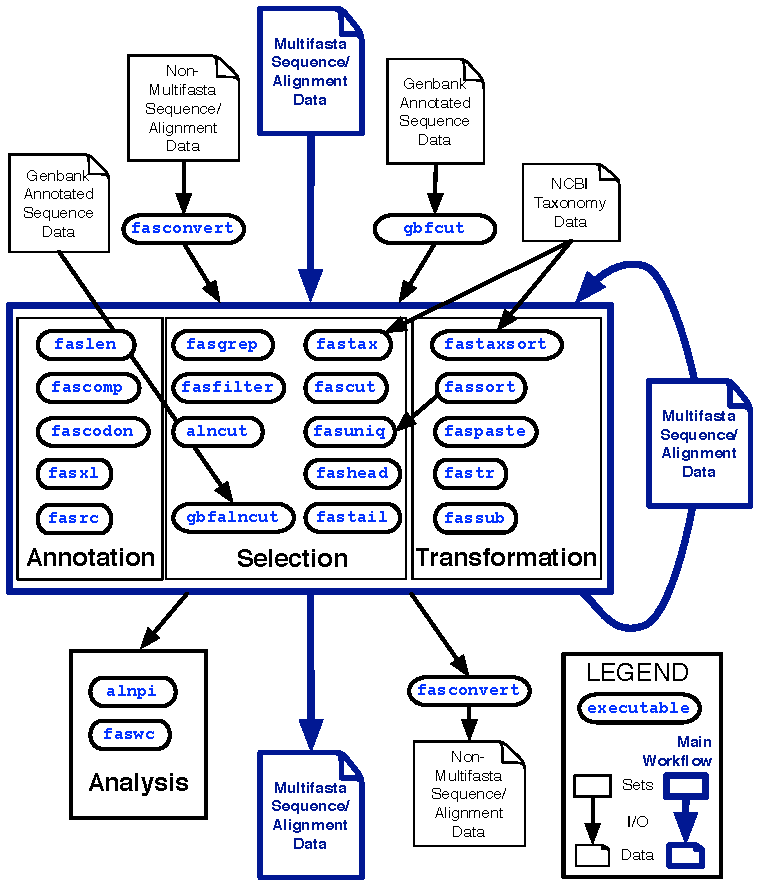
\includegraphics[width=4.5in]{FAST_v8}% This is a *.jpg file
\end{center}
\textbf{\refstepcounter{figure}\label{fig:01} Figure
  \arabic{figure}.}{ Overview of the first major release of FAST with
  data and workflow dependencies indicated.  Inputs to FAST tools are
  shown at the top of the figure with outputs at the bottom.  Outlined
  in blue is the primary working model, in which Multifasta sequence
  or alignment data is successively annotated, selected upon and
  transformed into new Mutifasta sequence alignment data, or fed into
  a utility in the {\bf analysis} category for tabular output of data
  summaries. Many of the utilities in the {\bf annotation} category
  are also optionally capable of tabular output.}
\end{figure}

\begin{figure}
\begin{center}
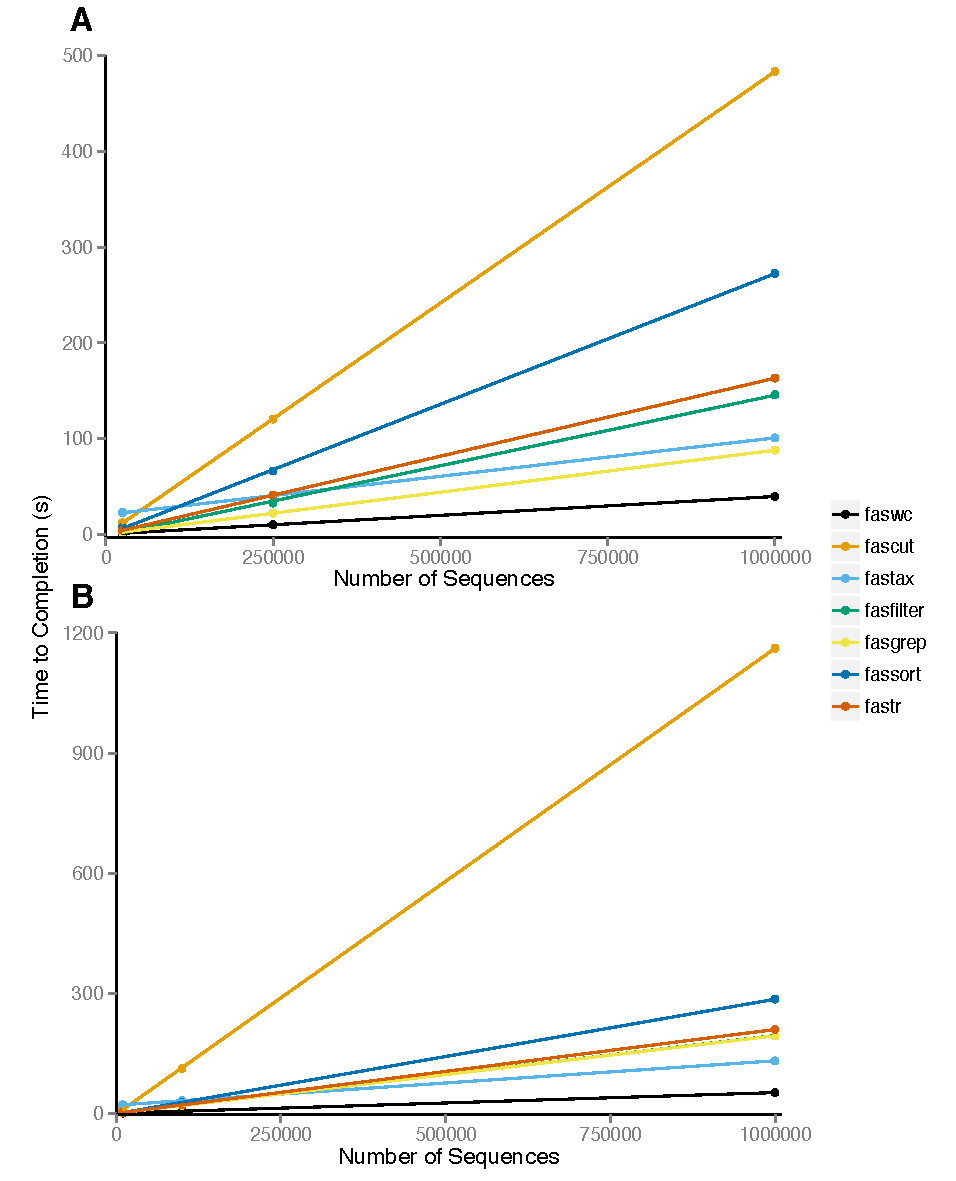
\includegraphics{Figure2}
\end{center}
\textbf{\refstepcounter{figure}\label{fig:02} Figure
  \arabic{figure}.}{ Average processor time of 100 repetitions
  required to complete analysis using indicated utility. Utilities
  were run on six datasets consisting of (a) 25000, 250000, and
  1000000 100bp sequences and (b) 10000, 100000, and 1000000 1000bp
  sequences. }
\end{figure}


\end{document}

%%% Local Variables:
%%% mode: latex
%%% TeX-master: t
%%% End:
